%File: formatting-instruction.tex
\documentclass[letterpaper]{article}
\usepackage{aaai}
\usepackage{times}
\usepackage{helvet}
\usepackage{courier}
\usepackage{graphicx}
\usepackage{amsmath}

\setlength{\pdfpagewidth}{8.5in}
\setlength{\pdfpageheight}{11in}
\pdfinfo{
/Title (Visualizing the Pulse of World Cities on Twitter)
/Author (Miguel Rios, Jimmy Lin)
}
\usepackage{color}
\newcommand{\red}[1]{\textcolor{red}{#1}}

\frenchspacing
%\pdfinfo{
%/Title (Formatting Instructions for Authors Using LaTeX)
%/Subject (AAAI Publications)
%/Author (AAAI Press)}
\newcommand{\ignore}[1]{}
\setcounter{secnumdepth}{0}  
 \begin{document}

% The file aaai.sty is the style file for AAAI Press 
% proceedings, working notes, and technical reports.
%
\title{Visualizing the ``Pulse'' of World Cities on Twitter}
\author{Miguel Rios \and Jimmy Lin\\
Twitter, Inc.\\
@miguelrios @lintool
}

%\author{Blinded for review}

%\nocopyright

\maketitle

\begin{abstract}
\begin{quote}
We present a large-scale analysis of activity on Twitter in 50 major
cities around the world throughout all of 2012. Our study consists of
two parts:\ First, we created heatmap visualizations, through which
periods of comparatively intense and sparse activity are readily
apparent---these visual patterns reflect diurnal cycles, cultural
norms, and even religious practices. Second, we performed a cluster
analysis of these activity patterns to identify groupings of cities
that are similar in the ways their inhabitants use Twitter. Not
surprisingly, cities cluster geographically, although we are able to
identify cross-cultural similarities as well.
\end{quote}
\end{abstract}

\section{Introduction}

Twitter has become an indispensable communications platform through
which hundreds of millions of users around the world keep up with
breaking news, share their thoughts, and connect with like-minded
individuals, 140 characters at a time. Aggregate patterns of user
behavior on Twitter tell us a lot about the ``pulse'' of the global
conversation. In this paper, we present a case study examining tweet
creation activity for 50 cities around the world throughout all of
2012. The analysis proceeds in two parts:\ First, we created heatmap
visualizations that show the intensity of Twitter activity in terms of
time of day and day of year. From these visualizations, the ``rhythm''
of activities in major cities becomes apparent:\ we see diurnal cycles
of waking and sleeping, weekly cycles of work and play, large seasonal
shifts in behavior, and even activity patterns that stem from
religious practices. Not surprisingly, we see large
differences in these patterns in different parts of the world,
reflecting cultural differences and the myriad ways that Twitter is
used. In the second part of our analysis, we treated these activity
patterns as ``fingerprints'' of each city and performed a clustering
analysis to quantify the similarities between individual cities and
groups of cities; these results are visualized in a dendrogram.

There are two reasons for presenting this work. First, we believe that our
results are intrinsically interesting, and we have not seen
large-scale analyses along these lines before. Such analyses are very
difficult to accomplish without access to all the data, since
any sampled stream becomes too sparse when focusing only on specific
geographic locations. In contrast, we have access to all tweets,
and thus we are confident that our findings are not artifacts
introduced by data sampling. Second, this work presents a case study
illustrating the role of visualization in data science. ``Big data''
and data science have gained prominence in both industry and academia,
but most of the discussion revolves around efficient algorithms for analyzing
terabytes to petabytes of data---for example, better join
algorithms. We feel that visualization deserves a more prominent role
in the discourse---after all, analyses on big data must
eventually be presented to humans for interpretation. Our case study
serves as an example of transforming terabytes on disk to pixels on screen.

\section{The Role of Visualizations}

Let us first elaborate on the second point, the role of
visualizations in data science. Ultimately, the data scientist's job
is to analyze massive amounts of data, interpret ``what the data
say'', and distill the bits into {\it actionable} insights:\ 
what web site elements to refine, what
features to develop, what markets to pursue, etc. To accomplish this,
data visualization is an indispensable tool. At a mundane level,
this involves dashboards to enable stakeholders to browse through
large amounts of multi-dimensional data, including interactive ``drill
downs'' and ``roll ups'', overlaid with projections and other derived
data. 

%This is quite similar to cube materialization in online
%analytical processing (OLAP) tasks for business intelligence, and is
%supported by a number of commercial off-the-shelf packages.

Beyond simple dashboards, data scientists often build one-off
visualizations that are the result of a specific task, usually a
business question. For example, in 2010 when Twitter was outgrowing
its datacenter footprint, we created a custom visualization that let
engineers interactively examine server utilization statistics along
with network bandwidth usage in order to better optimize resource
allocation.

Finally, we occasionally produce visualizations intended for public
consumption, which are presented on Twitter's blog. These are less
intended to generate insights for the business; rather, their primary
purpose is to highlight the ``pulse'' of the global conversation on
Twitter, often in reaction to major news events around the world.

Our study serves a combination of the second and third purposes. User
growth is an important priority for Twitter, and understanding
patterns of activity is a pre-requisite to facilitating growth. The
visualizations and analyses we present here were part of efforts to
better understand how Twitter users behave in different parts of the
world. Along the way, we discovered that many of our findings were
intrinsically interesting, and thus we have taken the additional step
of sharing our results with the community.

\begin{figure*}[p]
\centering
\setlength\fboxsep{0pt}
\setlength\fboxrule{0.25pt}
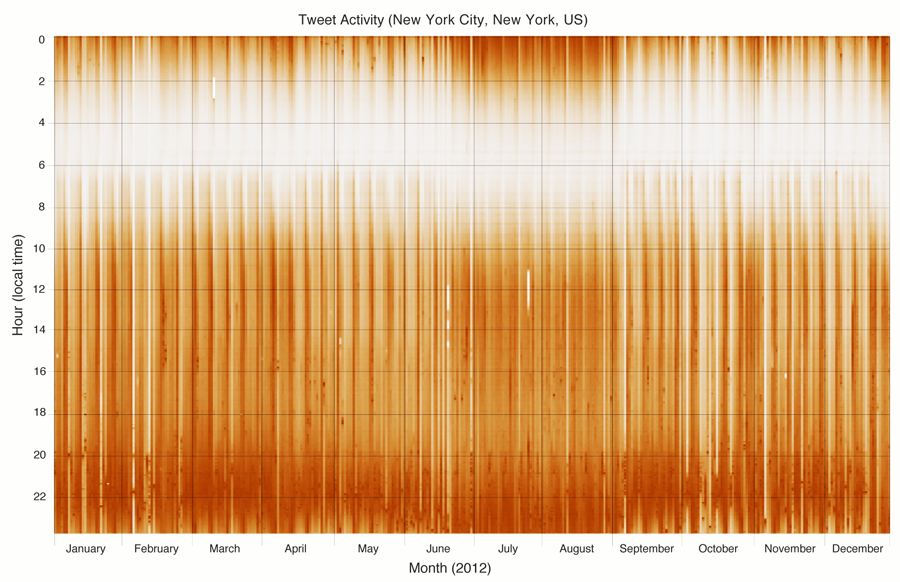
\includegraphics[width=0.45\linewidth]{heatmap_imgs/newyorkcity.png}
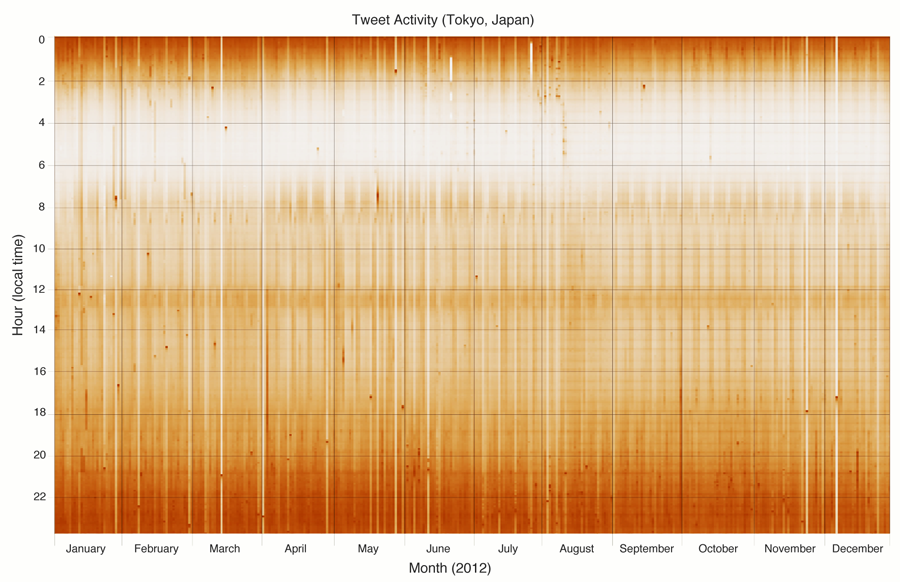
\includegraphics[width=0.45\linewidth]{heatmap_imgs/tokyo.png}
%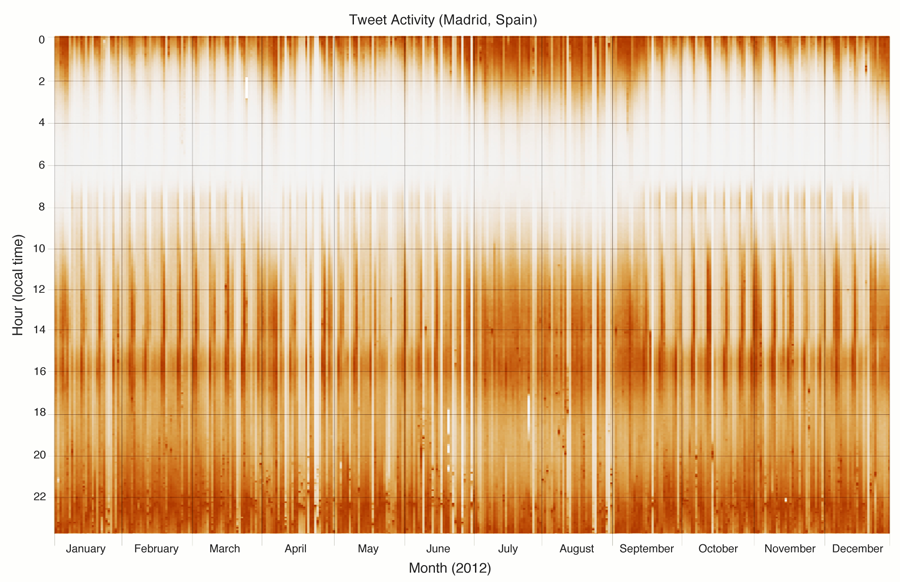
\includegraphics[width=0.45\linewidth]{heatmap_imgs/madrid.png}
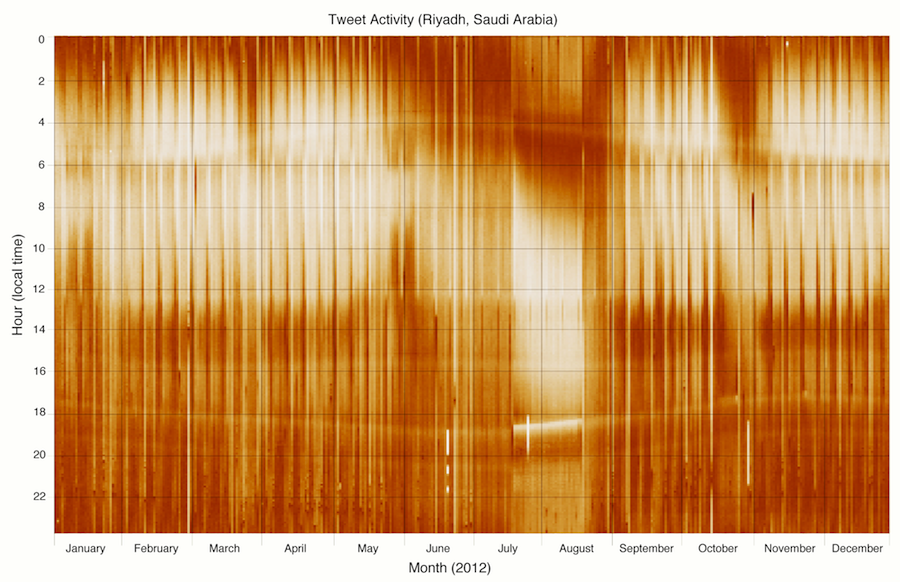
\includegraphics[width=0.45\linewidth]{heatmap_imgs/riyadh.png}
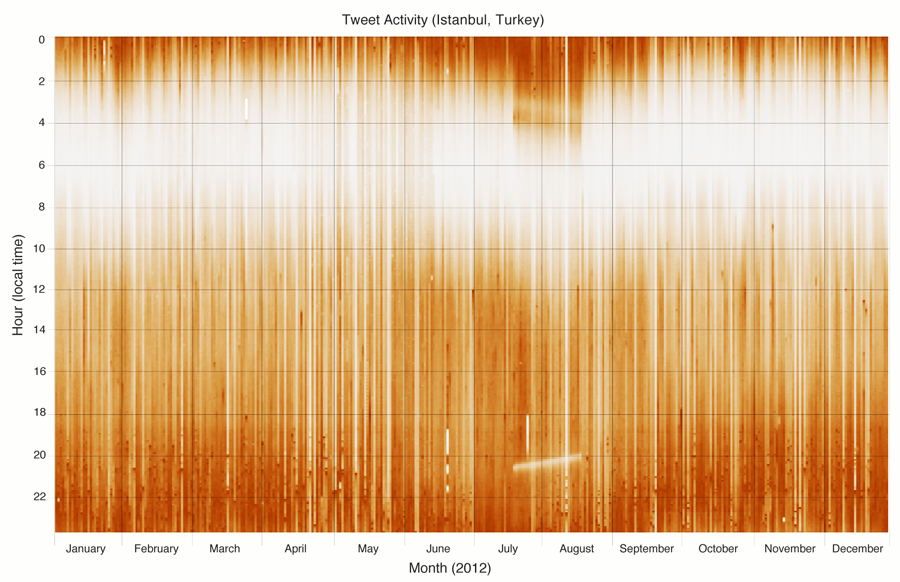
\includegraphics[width=0.45\linewidth]{heatmap_imgs/istanbul.png}
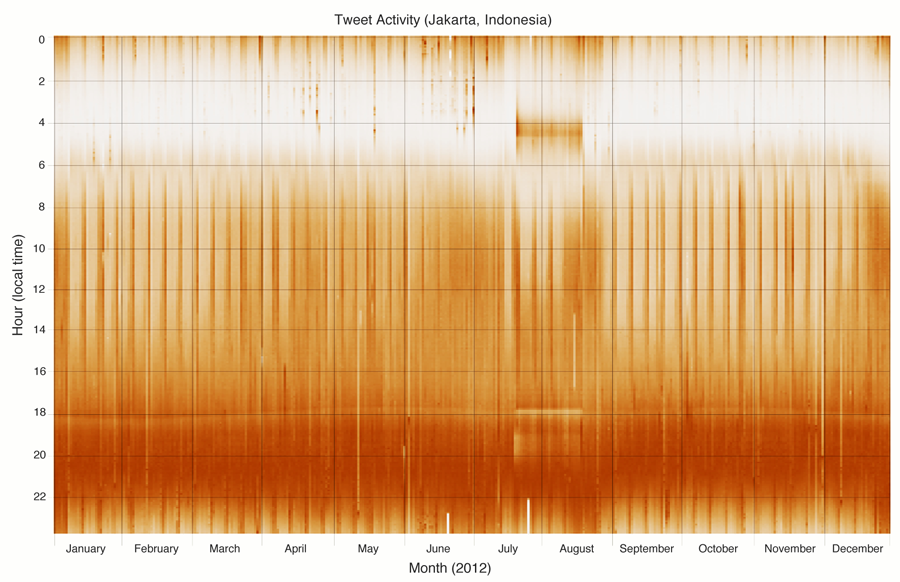
\includegraphics[width=0.45\linewidth]{heatmap_imgs/jakarta.png}
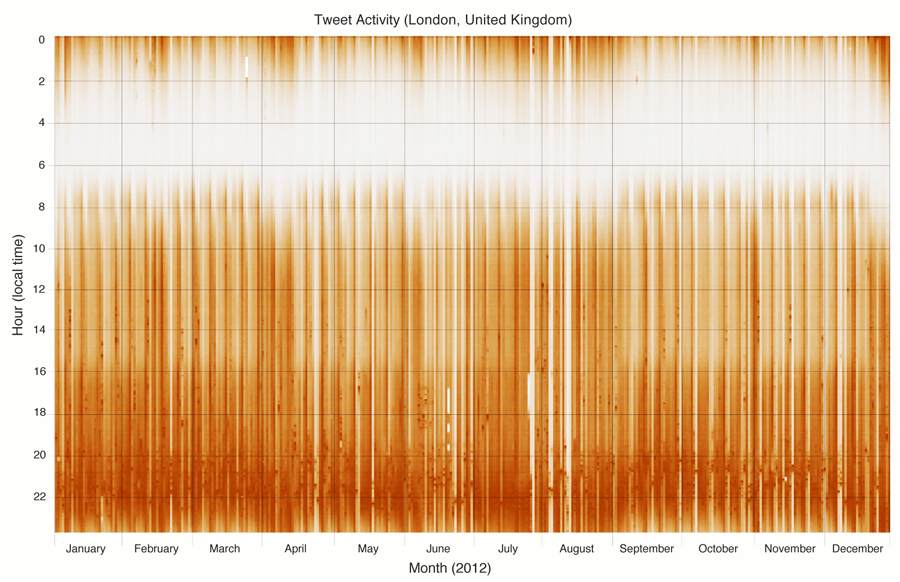
\includegraphics[width=0.45\linewidth]{heatmap_imgs/london.png}
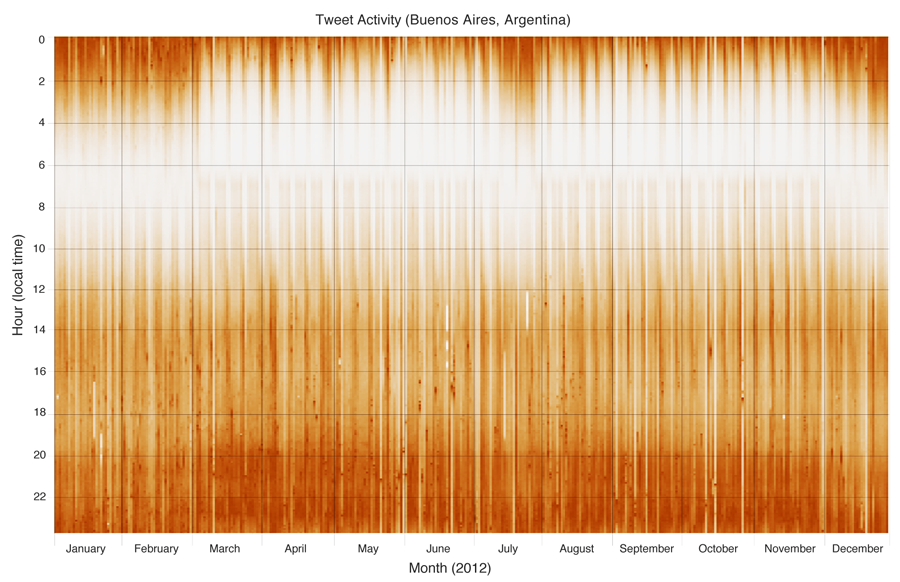
\includegraphics[width=0.45\linewidth]{heatmap_imgs/buenosaires.png}
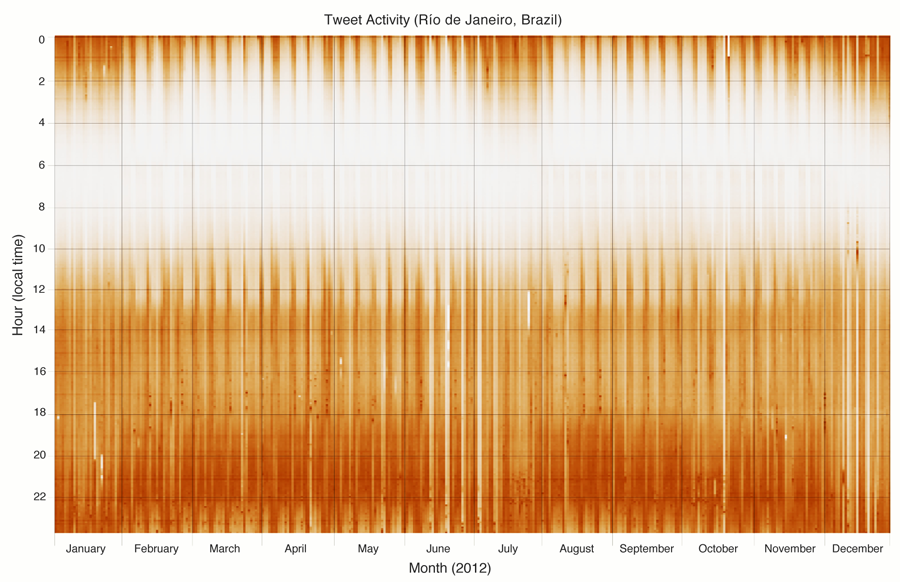
\includegraphics[width=0.45\linewidth]{heatmap_imgs/rio.png}
\caption{Heatmap visualizations of Twitter activity in eight cities around the world. The
  {\it x}-axes show day of year, and the {\it y}-axes show time of day (local time);
  darker shading indicates higher levels of activity.}
\label{viz:cities}
\end{figure*}

\begin{figure*}[t]
\centering
%\setlength\fboxsep{0pt}
%\setlength\fboxrule{0.25pt}
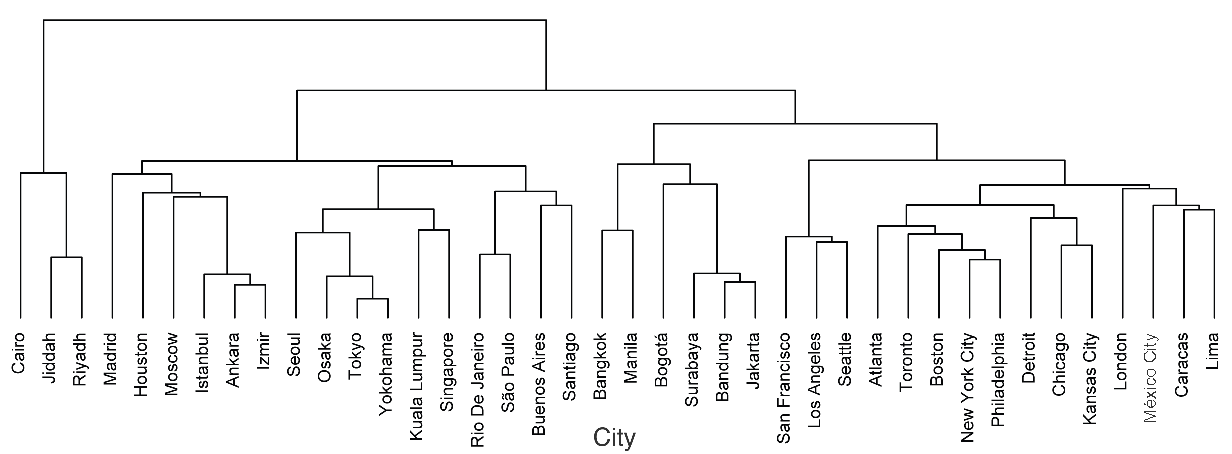
\includegraphics[width=0.95\linewidth]{dendrograms/dendogram_50_bottom_clean_shorter.pdf}
\caption{Hierarchical clustering of Twitter activity in 50 cities around the world.}
\label{viz:dendrogram}
\end{figure*}

\section{Data Preparation and Analysis}

Data preparation consisted of analyzing all public tweets posted in
2012 in our Hadoop-based data warehouse using Pig~\cite{Olston_etal_SIGMOD2008}. A more
detailed description of Twitter's analytics infrastructure can be found
in~\cite{Lin_Kolcz_SIGMOD2012}. Our analysis focused on the top 50
cities in terms of Twitter users. We divided each day into 10 minute
chunks and computed the number of tweets that were posted during each
interval as a way of quantifying activity. The values were normalized
between zero and one on a {\it per day} basis. This is an important
design decision because the total number of tweets changes day to day
and grows over time, but this treatment also results in a few
artifacts in the visualizations, as we shall discuss. For each city,
this gives us $365 \times 24 \times 6 = 53560$ data points.

\section{City by City Observations}

Figure~\ref{viz:cities} shows heatmap visualizations for eight of the
fifty cities that we examined. The {\it x}-axes show day of year, and
{\it y}-axes show time of day (local time); darker shading indicates higher levels
of activity. We examine each panel in turn:

\smallskip \noindent {\bf New York City.} What immediately jumps out
are the vertical stripe patterns which correspond to weekly cycles of
activity. Focusing on the morning hours, the pattern consists of a
wide region of comparatively darker shading followed by a narrow
region of lighter shading. This corresponds to users getting up earlier
during weekdays and later on weekends. The pattern changes later in
the day:\ we see a wide region of comparatively lighter shading followed by a
narrower region of darker shading. This is explained by users tweeting
less during work hours and comparatively more during the same period
of time on the weekends. Overall, Twitter activity is highest in the
evenings (both weekdays and weekends), and activity extends past
midnight on weekends.

In addition to the weekly cycles, we observe a
large seasonal shift. This corresponds to the school
calendar:\ for public schools, the final day of classes in the 2011--2012
school year was June 27, 2012, and the first day of classes in the
2012--2013 school year was September 6, 2012. The period of time in between marks
summer vacation for school children and
explains why we observe more activity past midnight and less activity
in the morning.

% NYC public school: 
% last day, 6/27/2012
% first day, 9/6/2012

The white empty space on March 11 corresponds to the beginning of
daylight saving time. Since all timestamps have been translated to
local time, that hour never ``existed'', since in the United States
users adjust their clocks to skip an hour. Note that there is no
corresponding artifact in November when daylight saving time ends---in
terms of local time, that hour ``repeats'', and we simply take the
average of both intervals. The other artifacts in the heatmap on June 21 and July
26 correspond to Twitter outages---they are present in the other panels as
well, but occur at different local times.

% Twitter outage on June 21, 2012
% July 26, 2012

\smallskip \noindent {\bf Tokyo.} Patterns of activity in Tokyo appear
very different from those in New York City. Although we still see the
striping pattern corresponding to weekly cycles, the contrast is far
lower. Compared to New York, users in Tokyo exhibit far less variation
in activity between weekends and weekdays. It appears that users
mostly tweet in the evening, with pockets of activity in the morning
and around noon (except on weekends). Also, we do not see any major
seasonal shifts. Overall, user behavior is remarkably consistent all
year-round.

\smallskip \noindent {\bf Riyadh.} In many ways, this was the most
surprising visualization of all the cities we looked at---so much so that initially
we thought there were data errors.
In the heatmap, we see five distinct bands:\ the top is convex in shape
with a peak in late June, the next two are mostly flat, and the bottom
two are concave with a trough also around June. These bands correspond
to the five daily prayers prescribed by Islam:\ the time of the first
(fajr) is determined by the sunrise, and the fourth (maghrib) and
fifth (isha) are determined based on sunset time, which explains
their distinct shapes.

Even more interesting, we see dramatic shifts in user activity between
July 19 and August 18, which corresponds to Ramadan. We notice a
substantial drop in activity around sunset during that time. Muslims
observe fasting during Ramadan from dawn until dusk---so that marks the first
opportunity to eat all day. We see that Twitter users collectively
take a break from tweeting to enjoy this opportunity!

\smallskip \noindent {\bf Istanbul.} Although Turkey is overwhelmingly
Muslim, the country is a secular republic. The ``prayer
bands'' that we see in Riyadh are not evident in the visualization,
but the behavior shift that occurs during Ramadan is still very
dramatic. Note that since Istanbul is at a higher latitude than
Riyadh, sunrise is earlier and sunset is later---this shows up clearly
in the heatmap as well. Finally, we note a slight difference in users'
behavior between Riyadh and Istanbul:\ Turkish users seem to stay up
later during Ramadan.

\smallskip \noindent {\bf Jakarta.} Indonesia is another
predominantly Muslim nation; on the whole, it is considered more
secular than Saudi Arabia but less so than Turkey. The activity
patterns, therefore, fall somewhere between the previous two
visualizations. We see the ``prayer band'' at sunset, but none of the
others are evident. Note that Jakarta lies at latitude 6 degrees north, close
to the equator, thus sunset time is relatively constant year
round. For that reason, we do not see the concave pattern present in
Riyadh.

Note that user behavior in Jakarta during Ramadan is different from
the two cities above. Although we do see the same pattern caused
by breaking fasting at sundown, users tend to go to sleep
{\it earlier}, and wake up right before sunrise.
This is the opposite from Istanbul, where
users stay up later. Overall, we see relatively little activity past midnight. Other
than Ramadan, there are no large-scale seasonal shifts.

%Very consistent, just like Tokyo, although Tokyo is much
%higher latitude, we don't see any artifacts of that.

\smallskip \noindent {\bf London.} In this visualization, we see
disruption to the normal rhythm of the city from late-July to
mid-August, which corresponds to the Olympics. The white stripes are
actually artifacts of the normalization procedure during data
processing. We see a much higher volume of tweets during the Olympic
events such that after normalization, all other time blocks
receive lighter shading in the heatmap.

\smallskip \noindent {\bf Buenos Aires.} Here, we see two distinct
periods, between end of February and mid-July, and between end of July
and mid-December, where there is substantially more activity in the
mornings. This corresponds to the school schedule in the southern
hemisphere, which, naturally, has opposite seasons compared to
the northern hemisphere. Correspondingly, the time between those
periods, we see greater activity later in the evenings---in fact,
extending far later into the early hours of the morning. We see
substantial activity until 3am and beyond, local time.

\smallskip \noindent {\bf Rio de Janeiro.} Just like for Buenos Aires,
we see patterns of activity that reflect the school schedule in the
southern hemisphere. Quite naturally, the two South American cities
have more similar activity patterns to each other than to other cities
around the world.
%Furthermore, of all the cities shown in Figure~\ref{viz:cities}, inhabitants
%of Rio de Janeiro and Buenos Aires seem to be more active past midnight
%than most of the others cities.

\section{Clustering Analysis}

The heatmap visualizations allow us to manually examine the activity
``fingerprint'' of each city. We followed up our observations with a
more quantitative cluster analysis. We treated
each temporal cell in the heatmap as a feature and performed
hierarchical clustering on the cities, using the complete linkage
approach. The results are shown as a dendrogram in
Figure~\ref{viz:dendrogram}.

The results confirm our visual analysis. We see nice clusterings of
cities in the same country: for example, Surabaya, Bandung, and
Jakarta in Indonesia; Rio de Janeiro and S\~{a}o Paulo in Brazil;
etc. What's even more remarkable is that for cities in the United
States, we see regional groupings---for example, the east coast cities
Boston, New York, and Philadelphia cluster together, as do the west
coast cities San Francisco, Los Angeles, and Seattle. Based on visual
observation, all American cities basically look the same, so the
clustering algorithm is picking up features that the eyes cannot detect.
There are a few oddities in the cluster analysis---for example, the
placement of Houston with other European cities such as Madrid and Moscow and the placement of
London near Mexico City, Caracas, and Lima. 
Interestingly, the clustering tells us that
Rio de Janeiro, S\~{a}o Paulo, Buenos Aires, and Santiago, which
are similar to each other, exhibit quite different activity patterns
from Caracas, Lima, and Bogot\'{a}, even though they are all South American cities.

\section{Conclusions and Future Work}

In this paper, we present a case study where terabytes of raw data (in
this case, tweet creation times) are transformed into visualizations
that reveal a great deal about differences in user behavior on Twitter
in different cities. We see diurnal cycles, weekly cycles, seasonal
shifts, and other large-scale behavior pattern changes. These activity
fingerprints are then further analyzed by clustering. We note that none
of these techniques are particularly sophisticated---heatmaps and
dendrograms are well-known visualization tools.
This goes to show that insightful visualizations do not need to be fancy:\ a data
scientist simply needs to apply the right tool for the job.

One area of future work is streamlining processes for creating
visualizations from big data. Currently, it is a very laborious and error prone
process, starting with Pig scripts that run on our Hadoop data
warehouse to distill terabytes of raw data into megabytes of refined
features. From there, we need to move the data into a separate tool
for the visualization. The clustering was performed with R, and final
preparation of the image panels required Photoshop. All told, around
half a dozen {\it different} tools must be brought to bear from
beginning to end. This is too complex and slow, and we as a community
need to develop better integrated workflows for insight generation.

\bibliographystyle{aaai} 
\small
\bibliography{heatmap}

\end{document}
